%sample file for Modelica 2015 Conference paper

\documentclass[11pt,a4paper,twocolumn]{article}
\usepackage{graphicx}
% uncomment according to your operating system:
% ------------------------------------------------
%\usepackage[latin1]{inputenc}    %% european characters can be used (Windows, old Linux)
\usepackage[utf8]{inputenc}     %% european characters can be used (Linux)
%\usepackage[applemac]{inputenc} %% european characters can be used (Mac OS)
% ------------------------------------------------
\usepackage[T1]{fontenc}     %% get hyphenation and accented letters right
\usepackage{mathptmx}        %% use fitting times fonts also in formulas
\usepackage{amsmath} %% Nice maths
\usepackage{doi}             %% Create cor­rect hy­per­links for DOI num­bers
\usepackage{booktabs}        %% Nice tables
\usepackage{hyperref}
\usepackage{color}
\usepackage[labelfont=bf, labelsep=period, font=small]{caption}  %% Get bold Figure/Table caption
               %% Set separator in figures to '.', set fontsize to small
\usepackage{authblk}         %% Prepare author and affiliation blocks
\usepackage{courier}         %% For proper courier fonts in texttt
\usepackage{listings}        %% For code sections
%\usepackage[bw]{dtsyntax}    %% For Modelica code

%% We are using biblatex instead of bibtex in order to support "online" references
\usepackage[backend=biber,
            style=authoryear,
            doi=false,
            isbn=false,
            ]{biblatex}
\addbibresource{impact.bib}
% We do not need the note fields printed
\AtEveryBibitem{%
  \clearfield{note}%
}
\usepackage{pifont}% http://ctan.org/pkg/pifont
\newcommand{\cmark}{\ding{52}}%
\newcommand{\xmark}{\ding{56}}%
\usepackage{dingbat}%
\usepackage{enumitem}% for tweaking lists

% do not change these lines:
\pagestyle{empty}                %% no page numbers!
\usepackage{geometry}            %% please don't change geometry settings!
\geometry{left=20mm, right=20mm, top=25mm, bottom=25mm, noheadfoot}

\hypersetup{%
  pdftitle = {Where impact got going},
  pdfauthor = {Michael Tiller and Dietmar Winkler},
  pdfsubject = {11th International Modelica Conference 2015},
  pdfkeywords = {Modelica, package manager, GitHub, dependency management, golang},
  hidelinks,
  pdfpagelayout=SinglePage}

\renewcommand{\normalsize}{\fontsize{10.5pt}{12.3pt}\selectfont}
\renewcommand{\small}{\fontsize{9.5pt}{11.1pt}\selectfont}
\renewcommand{\footnotesize}{\fontsize{8.5pt}{9.9pt}\selectfont}

%% Modelica code configuration
% \lstset{language = Modelica,
%        basicstyle=\fontsize{9pt}{10.5pt}\selectfont,
%        backgroundcolor = \color{white}}

% usefull commands
\newcommand{\myr}{\textsuperscript{\textregistered}}
\newcommand{\ud}{\mathrm{d}}
\newcommand{\matx}[1]{\mathbf{#1}}
\newcommand{\impact}{\texttt{impact}} % impact is going to get used quite a lot :)
\newcommand{\code}[1]{\texttt{#1}} % make quoting code text a bit simpler


% begin the document
\begin{document}
\thispagestyle{empty}

\title{\textbf{Where \impact\ got \emph{go}ing}}
\renewcommand\Authfont{\large}        %% Set author font
\renewcommand\Affilfont{\normalsize}       %% Set affiliation font
\renewcommand\Authsep{\quad}                     %% Set text between authors names
\renewcommand\Authand{\quad}                     %% Set text between authors names
\renewcommand\Authands{\quad}                    %% Set text between authors names
\author[1]{Michael Tiller}
\author[2]{Dietmar Winkler}
\affil[1]{\href{http://xogeny.com}{Xogeny Inc.}, USA, {\small \href{mailto:michael.tiller@xogeny.com}{\nolinkurl{michael.tiller@xogeny.com}}}}
\affil[2]{\href{http://www.hit.no}{Telemark University College},  Norway, {\small\href{mailto:dietmar.winkler@hit.no}{\nolinkurl{dietmar.winkler@hit.no}}}}

% \title{\textbf{Int. Modelica Conf. 2015 Paper Title}}
% \author{{\large
% Author Name$^1$ \quad Author Name$^1$ \quad Author Name$^2$\vspace{2mm}\\
%   {}$^1$Department, University, Country, \textsf{\{name1,name2\}@university.org}\\
%   {}$^2$Company, Contry, \textsf{name3@company}}


\date{} % <--- leave date empty
\maketitle\thispagestyle{empty} %% <-- you need this for the first page
\abstract{%

  This paper discussed the \code{impact} package manager.  The primary
  goal of this project is to support the development of a healthy
  eco-system around Modelica.  For many other languages, the existance
  of an easy to use package manager has made it easier for people to
  explore and adopt those languages.  We seek to bring that same kind
  of capability to the Modelica community by incorporating useful
  features from other package managers like \code{bower}, \code{npm},
  \emph{etc.}

  This paper is an update on the status of the \code{impact} package
  manager which was discussed previously in \parencite{impact1}.  This
  latest version of \code{impact} involves a complete rewrite that
  incorporates a more advanced dependency resolution algorithm.  That
  dependency resolution will be discussed in depth along with many of
  the subtle issues that arose during the development of this latest
  version of \code{impact}.  Along with a superior dependency resolution
  scheme, the new version of \code{impact} is much easier to install
  and use.  Futhermore, it includes many useful new features as well.

}

\noindent\emph{Keywords: Modelica, package management, GitHub, dependency resolution, golang}

\section{Introduction}

\subsection{Motivation}

The motivation behind the \code{impact} project is to support two
critical aspects of library development.  The first is to make it very
easy for library developers to \emph{publish} their work.  The second
is, at the same time, to make it easy for library consumers to both
find and install published libraries.

We also feel it is important  to reinforce best practices with respect
to model development.   For this reason, we have  made version control
an integral  part of  our solution.   Rather than  putting users  in a
position to have  to figure out how to make  \code{impact} work with a
version control  system, we've build \code{impact}  around the version
control system.   Not only  do users not  have to find  a way  to make
these technologies work together,  \code{impact} actually nudges those
not using  version control  toward solutions that  incorporate version
control.  In this way, we hope to demonstrate to people the advantages
of both \code{impact} and version control and establish both as ``best
practices'' for model development.

By creating a tool that makes it easy to both publish and install
libraries, we feel we are creating a critical piece of the foundation
necessary to establish a \textbf{healthy ecosystem} for model
development.

\subsection{History}

Earlier, we mentioned that \code{impact} has been completely
rewritten.  In fact, the very first version of \code{impact} was just
a single Python script for indexing and installing Modelica
code\parencite{impact-gist}.  It eventually involved into a multi-file
package that could be installed using the Python package management
tools.

\section{Requirements}

After building the original Python version, we gave some thought to
what worked and what didn't work well.  One issue we ran into almost
immediately was the complexity of installing the Python version of
\code{impact}.  Python is unusual in that it has two package managers,
\code{easy\_install} and \code{pip}.  It comes with
\code{easy\_install}, but \code{pip} is the more capable package
manager.  So in order for someone to install \code{impact}, they first
needed to install Python, then install \code{pip} and then install
\code{impact}.  This was far too complicated.  So we wanted to come up
with a way for people to install \code{impact} \textbf{as a simple
  executable} without any runtime or prerequisites.

Another issue we ran into with the Python version was the fact that
there are two different and incompatible versions of Python being used
today.  Trying to support both was an unnecessarily inefficient use of
resources.  For this reason, we felt we needed to move away from
Python altogether.

We also had some difficulties in the Python version with support for
SSL under Windows \parencite{python-ssl}.  Because we were doing lots of
``crawling'' (more on this shortly), we needed a platform that
provided \textbf{solid HTTP client support}.

Although most users Modelica run their development tools and
simulations under Windows, there are several tools that support OSX
and Linux as well as Windows.  So as to not neglect users of those
tools and to support more cross-platform options, we also wanted to be
able to \textbf{compile \code{impact} for all three major platforms}.

Furthermore, we wanted to provide a simple executable for all
platforms without having to have actual development machines for each
of these different platforms.  For this reason, \textbf{cross
  compilation} between different platforms was an important
consideration was well.

Of course, we also wanted to have \textbf{good performance}.  For most
package management related functions, the speed of the internet
connection is probably the biggest limitating factor.  So CPU
performance wasn't that high on the list.  But, as we shall discuss
shortly, the computational complexity of the dependency resolution
algorithm we implemented could lead to some computationally intensive
calculations for complex systems of dependencies.

For these reasons, we ultimately rewrote \code{impact} in Go.  Go is a
relatively new language from Google that stresses simplicity in
language semantics but, at the same time, provides a fairly complete
standard library.  You can think of Go as being quite similar to C
with support for extremely simple object-oriented functionality,
automatic garbage collection and language level support for CSP-based
concurrency.  With Go, we were able to satisfy all the requirements
above.

\section{Version Numbering}
\label{sec:numbers}

Before we dive into all the details associated with crawling,
indexing, resolving and installing, it is useful to take a moment to
briefly discuss versioning.  Modelica supports the notion of versions
through the use of the \texttt{version} and \texttt{uses} annotations.  These two
annotations allow libraries to explicitly state what version they are
and what versions of other libraries they use, respectively.

But there is one complication to the way Modelica deals with versions.
In Modelica, a version is simply a string.  This by itself isn't a
problem.  But it becomes a problem, as we will discuss in greater
detail shortly, when you need to understand relationships between
version.  In particular, there are two important things we would like
to determine when dealing with version numbers.  The first is an
unambiguous ordering of versions.  In other words, which, of any two
versions, is the ``latest'' version?  The second is whether a newer
version of a library is ``backwards compatible'' with a previous
version.  These are essential questions when trying to resolve
dependencies and the current string based approach to versions in
Modelica is not semantically rich enough to help us answer either of
these.

This issue is not unique to the Modelica world.  These same questions
have been asked for a very long time and various approaches have been
invented to deal with answering these questions.  One recent and
widely used approach is to employ what is called \textbf{semantic
  versioning}\parencite{semver}.  Semantic versioning is pretty much what
it sounds like, an approach to defining version numbers where the
version numbers have very explicit meanings associated with them.

A very simple summary of semantic versioning would be that \textbf{all}
versions have exactly three numerical components, a major version
number, a minor version number and a patch.  A semantic version must
have all of these numbers and they must be \texttt{.}-separated.  For this
reason, the following versions are not legal semantic version numbers:
\code{1}, \code{1a}, \code{1.0}, \code{1.0-beta5}, \code{4.0.2.4096}.
Each of these number means something.  If you make a non-backward
compatible change, you must increment the major version.  If you make
a backward compatible version, you must increment the minor version.
If you make a change that should be completely compatible with the
previous version, you increment only the patch version.

There are additional provisions in semantic versioning to handle
pre-release versions as well as build annotations.  We will not
discuss those semantics here, but they are incorporated into our
implementation's treatment of version numbers.

Our use of semantic versioning is aligned with our goal of strongly
encouraging best practices.  It is important to point out that the use
of semantic versions is completely legal in Modelica.  In other words,
Modelica allows a wider range of interpretations of version numbers.
By using semantic versions, we narrow these interpretations but we
feel that this narrowing is much better for the developer since it
also provides meaning to the version numbers assigned to a library.

However, because Modelica libraries are free to use nearly any string
as a version number, we need to find a way to ``bridge the gap''
between past usage and the usage we are encouraging moving forward.
Although internally \code{impact} understands \textbf{only} semantic
versions, it is still able to work with nearly all existing Modelica
libraries.  This is achieved through a process of ``normalizing''
existing versions.  When \code{impact} comes across versions that are
not legal semantic versions, it attempts to create an equivalent
semantic version representation.  For example, a library with a
version string of \code{1.0} would be represented by the semantic
version \code{1.0.0}.

For this normalization to work, it is important to make sure that the
normalization is performed \emph{both} on the version number associated
with a library and on the version numbers of the libraries used.  In
other words, it must be applied consistently to both the
\code{version} and \code{uses} annotations.

\section{Indexing}

As mentioned previously, there are two main functions that
\code{impact} performs.  The first is making it easy for library
developers to publish their libraries and the other is making it easy
for consumers to find and install those same libraries.  Where these
two needs meet is the library index.  The index is \textbf{built} by
collecting information about publish libraries.  The same index is
\textbf{used} by consumers searching for information about available
libraries.

Building the index involves crawling through repositories and
extracting information about libraries that those repositories
contain.  In the following section we will discuss this crawling
process in detail and describe the information that is collected and
published in the resulting index.

\subsection{Sources}

Currently, \code{impact} only supports crawling GitHub\parencite{github}
repositories.  It does this by usin the GitHub API\parencite{gh-api} to
search through repositories associated with particular users and to
look for Modelica libraries stored in those repositories.  We will
shortly discuss exactly how it identifies Modelica libraries.  But
before we cover those details it is first necessary to understand
which \emph{versions} of the repository it looks in.

Each change in a Git repository involves a \emph{commit}.  That commit
affects the contents of one or more files in the repository.  During
development, there are frequent commits.  To identify specific
versions of the repository, a tag can be associated with that
version.  Each tag in the repository history that starts with a
\code{v} and is followed by a semantic version number is analyzed by
\code{impact}.

\subsection{Repository Structure}

For each version of a repository tagged with a semantic version
number, \code{impact} inspects to contents of that version of the
repository looking for Modelica libraries.  There are effectively two
ways that \code{impact} finds Modelica libraries in a repository.  The
first is to check for libraries in ``obvious'' places that conform to
some common conventions.  For cases where such conventions are
insufficient, \code{impact} looks for a file named \code{impact.json}
to explicitly provide information about the repository.

\subsubsection{Conventions}

With respect to \code{impact}, the following is a list of ``obvious''
places that \code{impact} checks for the presence of Modelica
libraries:

\begin{itemize}[noitemsep]
  \item \textbf{\code{./package.mo}} The entire repository is treated as a Modelica
    package whose name is the name of the repository.

  \item \textbf{\code{./<dirname>/package.mo}} or\\  \textbf{\code{./<dirname>
      <ver>/package.mo}} The directory \code{<dirname>} is presumed to
    be a Modelica package.  The name of the library is determined by
    parsing the \code{package.mo} file.

  \item \textbf{\code{./<filename>.mo}} or\\ \textbf{\code{./<filename> <ver>.mo}} The
    file \code{./<filename>.mo} is a file containing a Modelica
    library.  The name of the library is determined by parsing the
    file.
\end{itemize}

As can be seen from these conventions, only files and directories that
exist at the root level are checked for Modelica content.

\subsubsection{\code{impact.json}}
\label{sec:dirinfo}

For various reasons, library developers may not wish to conform to the
repository structure patterns discussed previous.  Furthermore, there
may be additional information they wish to include about their
libraries.  For this reason, a library developer can include an
\code{impact.json} file in the root of the repository directory that
provides additional information about the contents of the repository.
For example, a repository may contain two or more Modelica libraries
in subdirectories.  The \code{impact.json} file allows information
about the storage location of each library in the repository to be
provided by the library developer.  Furthermore, the author may wish
to include contact information beyond what can be extracted from
information about the repository and its owner.  These are just a few
use cases for why an \code{impact.json} file might be useful for
library developers.  A complete schema for the \code{impact.json} file
can be found later in Section~\ref{sec:dirinfo_schema}.

\subsection{Handling Forks}

The Modelica specification implicitly assumes that each library is
uniquely identified by its name.  This name is used in both the
\code{version} and \code{uses} annotations as well as any references
in Modelica code (e.g., \code{Modelica} in \code{Modelica.SIunits}).
This assumption works well when discussing libraries currently loaded
into a given tool.  But when you expand the scope of your
``namespace'' to include all libraries available from multiple
sources, the chance for overlap becomes possible and must be dealt
with.

Previously, we mentioned the importance of supporting best practices
in model development and the specific need to accomodate version
control as part of that process.  Up until now, we have leveraged
version control to make the process of indexing and collection
libraries easier.  However, version control does introduce one
complexity as well.  That complexity is how to deal with \emph{forks}.

A fork occurs when there are multiple perspectives on how development
should progress on a given project.  In some cases, rather than
reconciling these different perspectives, developers decide to proceed
in different directions.  When this happens, the project becomes
``forked'' and there are then (at least) two \textbf{different} libraries
being developed in parallel.  Each of these libraries may share a
common name and perhaps even the same version numbers but still be
fundamentally different libraries.

A fork can arise for another, more positive, reason.  When someone
improves a library they may not have permission to simply fold their
improvement back into the original library.  On GitHub in particular,
it is extremely common for a library to be forked simply to enable a
third-party to make an improvement.  The author of the improvement
then sends what is called a \emph{pull request} to the library author
asking them to incorporate the improvement.  In such a workflow, the
fork is simply a temporary measure to support concurrent development.
Once the pull request is accepted, the fork can be removed entirely.

Regardless of why the fork occurs, it is important that \code{impact}
accomodates cases where forking occurs.  This is because forking is a
very common occurrence in a healthy eco-system.  It indicates progress
and interest and we should not do anything to stiffle either of
these.The issue with forking is that the same name might be used by
multiple libraries.  In such cases, we need a better way to uniquely
identify libraries.

For this reason, \code{impact} records \textbf{not only the library name,
  but also a URI associated with each library}.  In this way, the URI
serves as a completely unambiguous way of identifying different
libraries.  While two forks may have the same name, they will never
have the same URI\@.

\subsection{Schema}

We've mentioned the kinds of information \code{impact} collects while
indexing as well as the kind of information that might be provided by
library developers (via \code{impact.json} files).  In this section,
we will provide a complete description of information used by
\code{impact}.

\subsubsection{\code{impact\_index.json}}
\label{sec:index_schema}

The root of an \code{impact\_index.json} file contains only two
elements:

\begin{description}[noitemsep]
  \item[\code{version}] A string indicating what version of impact
    generated the index.  The string is, of course, a semantic
    version.
  \item[\code{libraries}] The libraries field is an array.  Each
    element in the array describes a library that was found.  \textbf{The
      order of the elements is significant}.  Libraries that occur
    earlier in the list take precedence over libraries that appear
    later.  This is important in cases where libraries have the same
    name.
\end{description}

For each library in the \code{libraries} array, the following
information may be present:

\begin{description}[noitemsep]
  \item[\code{name}] The name of the library (as used in Modelica)
  \item[\code{description}] A textual description of the library
  \item[\code{stars}] A way of ``rating'' libraries.  In the case of
    GitHub, this the number of times the repository has been starred.
    But for other types of sources, other metrics can be used.
  \item[\code{uri}] A URI to uniquely identify the given library (when
    it shares a common \code{name} with another library)
  \item[\code{owner\_uri}] A URI to uniquely identify the owner of the
    library
  \item[\code{email}] The email address of the owner/maintainer of the
    library
  \item[\code{homepage}] The URL for the library's homepage
  \item[\code{repository}] The URI for the library's source code
    repository
  \item[\code{format}] The format of the library's source code
    repository (e.g., Git, Mercurial, Subversion, \emph{etc.})
  \item[\code{versions}] This is an object that maps a semantic
    version (in the form of a string) to details associated with that
    specific version
\end{description}

The details associated with each version are as follows:

\begin{description}[noitemsep]
  \item[\code{version}] A string representation of the semantic
    version (\emph{i.e.,} one that is identical to the key).
  \item[\code{tarball\_url}] A URL that points to an archive of the
    repository in \code{tar} format.
  \item[\code{zipball\_url}] A URL that points to an archive of the
    repository in \code{zip} format.
  \item[\code{path}] The location of the library within the
    repository.
  \item[\code{isfile}] Whether the Modelica library is stored as a
    file (\code{true}) or as a directory (\code{false})
  \item[\code{sha}] This is a hash associated with this particular
    version.  This is currently recorded by \code{impact} during
    indexing but not used.  Such a hash could be useful for caching
    repository information locally.
  \item[\code{dependencies}] This is an array listing the dependencies
    that this particular version has on other Modelica libraries.
    Each element in this array is an object with one field,
    \code{name}, giving the name of the required library and another
    field, \code{version}, which is the \textbf{semantic version} of that
    library represented as a string (see previous discussion on
    normalization in~\ref{sec:numbers}).
\end{description}

\subsubsection{\code{impact.json}}
\label{sec:dirinfo_schema}

As mentioned previously in Section~\ref{sec:dirinfo}, each directory
can include a file named \code{impact.json} that provides explicit
information about Modelica libraries contained in that repository.
The root of the \code{impact.json} file contains the following
information:

\begin{description}[noitemsep]
  \item[\code{owner\_uri}] A link to information about the libraries
    owner
  \item[\code{email}] The email address of the owner or maintainer
  \item[\code{alias}] An object that whose keys are the names of
    libraries and whose associated values are the unique URIs of those
    libraries.  This information can, therefore, be used to
    disambiguate between dependencies where there may be multiple
    libraries with that name.
  \item[\code{libraries}] This is an array where each element contains
    information about a library present in the repository.
\end{description}

For each library listed in the \code{libraries} field, the following
information may be provided:

\begin{description}[noitemsep]
  \item[\code{name}] The name of the library
  \item[\code{path}] The path to the library
  \item[\code{isfile}] Whether the entity pointed to by \code{path} is
    a Modelica library stored as a file (\code{true}) or as a
    directory (\code{false}).
  \item[\code{issues\_url}] A link pointing to the issue tracker for
    this library
  \item[\code{dependencies}] An explicit list of dependencies for this
    library (if not provided, the list will be based on the
    \code{uses} annotations found in the package definition).
\end{description}

For each dependency, the following information should be provided:

\begin{description}
  \item[\code{name}] Name of the required library
  \item[\code{uri}] Unique URI of the required library
  \item[\code{version}] \textbf{Semantic version} number of the required
    library (represented as a string)
\end{description}

\section{Installation}

The previous section focused on how \code{impact} collects information
about available libraries.  The main application for this information
is support installation of those libraries.  In this section, we'll
discuss the installation side of using \code{impact}.

\subsection{Dependency Resolution}

\subsubsection{Background}

To understand the abstract problem behind the concept of a dependency,
we refer to the formal study undertaken in \parencite{boender2011formal}.
There, a repository is defined as a triple $(R,D,C)$ of a set of
packages $R$, a dependency function $D : R \rightarrow
\mathcal{P}(\mathcal{P}(R))$, and a \emph{conflict relation} $C
\subseteq R \times R$.  At that level, version numbers have been
abstracted to (distinguishable) packages: Every version yields a
distinctive package $p \in P$.

The dependency function $D$ maps a package $p$ to sets of sets of
packages $d \in D(p)$, where each set represents a way to provide one
required required feature of $p$.  In other words: If for each $d \in
D(p)$ at least one package in $d$ is installed, it is possible to use
$p$.

Currently, there is no way to express \emph{conflicts} directly in a
Modelica package.  However, due to the existance of external libraries
(which could conflict in arbitrary ways), it is likely that such a
need will arise in the future.  Additionally, current Modelica makes
it impossible to refer to two different versions of a library from the
same model.  Hence, we consider different versions of the same package
conflicting (\code{impact} can will only install one version of each
package in a given context).

The dependency resolution of \code{impact} fits into Boender's model.
Therefore, the conclusions drawn in \parencite{boender2011formal} can be
applied to \code{impact} as well:

The set of packages \code{impact} installs for a given project needs to
fulfill two properties, Boender calls \emph{abundance} and \emph{peace}.
Informally, abundance captures the requirement that all dependencies
be met while peace avoids packages that are in conflict with each
other.  A set of packages that is peaceful and abundant is called
\emph{healthy} and a package $p$ is called \emph{installable} w.r.t.\ a
given repository if and only if there exists a healthy set $I$ in said
repository such that $p \in I$.

The problem of finding such an installable set is however a hard one.
In fact, Boender proves by a simple isomorphism between the boolean
satisfiability problem and the dependency resolution that finding such
a set is NP-hard.  Fortunately, for the current typical problem size,
this isn't really an issue.

\subsubsection{Resolution Algorithm}
\label{sec:algorithm}

The indexing process collects quite a bit of information about
available libraries.  Most of the complexity in implementing the
installation functionality in \code{impact} is in figuring out
\textbf{what} to install.  And most of that complexity is in finding a set
of versions for the required libraries that satisfy all the dependency
relations.  This process is called dependency resolution.

The resolution algorithm starts with a list of libraries that the user
wants to install.  In some cases, this may be a single library but, in
general, the list can be of any length.  For each library in the list,
the user may specify a particular version of the library they wish to
install, but this isn't mandatory.  One important point here is that
we refer to this as a \emph{list}, not a set.  Order is significant
here.  The libraries that appear first are given a higher priority
than those that appear later.

Let's explain why this priority is important.  Consider a user who
wishes to install libraries \code{A} and \code{B}.  If the user has
not explicitly specified what version of each library they are
interested in, \code{impact} assumes the user wants the latest
version.  But what if the latest version of \emph{both} cannot be
used.  To understand this case, consider the following constraints:

\begin{description}
  \item \code{A:1.0.0} uses \code{B:2.0.0}
  \item \code{A:2.0.0} uses \code{B:1.0.0}
\end{description}

where \code{A:1.0.0} means version \code{1.0.0} of library \code{A}.
This example is admittedly contrived, but the underlying issue
is not.  We can see here that if we want the latest version of
\code{A}, we cannot also use the latest version of \code{B} (and
\emph{vice versa}) while still honoring the constraints above.  The
ordering of the libraries determines how we ``break the tie'' here.
Since \code{A} appears first, we assume it is more important to have
the latest version of \code{A} than to have the latest version of
\code{B}.

Let's take this extremely simple example to outline how the resolution
algorithm would function in this case.  In later sections, we'll
introduce additional complexities that must be dealt with.

If a user asks for libraries \code{A} and \code{B} to be installed,
the question that the dependency algorithm has to answer is \textbf{which
  versions} do we use.  Assuming that each library has a version
\code{1.0.0} and \code{2.0.0}, then each ``variable'' in this
problem has two possible values.  The following table essentially
summarizes the possibilities:
{\small
\begin{center}
\begin{tabular}{cc}
  Version of \code{A} & Version of \code{B} \\
  \code{1.0.0} & \code{1.0.0} \\
  \code{1.0.0} & \code{2.0.0} \\
  \code{2.0.0} & \code{1.0.0} \\
  \code{2.0.0} & \code{2.0.0} \\
\end{tabular}
\end{center}
}
This is a simple enumeration of the possibilities.  But
\emph{remember}, we assume the user wants the most recent version
\emph{and} we assume \code{A} is more important than \code{B}.  Semantic
versioning provides us with a basis for determining which version is
more recent.  Given these we reorder these combinations so that the
most desirable combinations appear first and the least desirable
appear last:
{\small
\begin{center}
\begin{tabular}{cc}
  Version of \code{A} & Version of \code{B} \\
  \code{2.0.0} & \code{2.0.0} \\
  \code{2.0.0} & \code{1.0.0} \\
  \code{1.0.0} & \code{2.0.0} \\
  \code{1.0.0} & \code{1.0.0} \\
\end{tabular}
\end{center}
}
Now we see the \code{impact} of the dependency constraints.  Specifically,
the first (most desirable) combination in this table does not satisfy
the dependency constraints (\emph{i.e.,} \code{A:2.0.0} does not work
with \code{B:2.0.0}).  If we eliminate rows that violate our
dependency constraints, we are left with:
{\small
\begin{center}
\begin{tabular}{cc}
  Version of \code{A} & Version of \code{B} \\
  \code{2.0.0} & \code{1.0.0} \\
  \code{1.0.0} & \code{2.0.0} \\
\end{tabular}
\end{center}
}
In summary, we order the combinations by their desirability
(considering both the relative priority of the libraries and their
version numbers) and then we eliminate combinations that don't satisfy
our dependency constraints.

This gives an overview of how the algorithm works conceptually.  But,
as you may have guessed, the problem is not quite this simple.
Consider now a slightly more complex case with the following
dependencies:
{\small
\begin{center}
\begin{tabular}{llcl}
  \textbf{1} &\code{A:3.0.0} &uses &\code{B:1.2.0} \\
  \textbf{2} &\code{A:3.0.0} &uses &\code{C:1.1.0}\\
  \textbf{3} &\code{B:1.2.0} &uses &\code{C:1.2.0}\\
  \textbf{4} &\code{A:2.0.0} &uses &\code{B:1.1.0}\\
  \textbf{5} &\code{A:2.0.0} &uses &\code{C:1.0.0}\\
  \textbf{6} &\code{B:1.1.0} &uses &\code{C:1.1.0}\\
  \textbf{7} &\code{A:1.0.0} &uses &\code{B:1.0.0}\\
  \textbf{8} &\code{A:1.0.0} &uses &\code{C:1.0.0}\\
  \textbf{9} &\code{B:1.0.0} &uses &\code{C:1.0.0}
\end{tabular}
\end{center}
} Now we have three variables we need to solve for, \code{A}, \code{B}
and \code{C}.  For each variable, we have three possible values.  As
we've already described, newer versions are prefered over older
versions while searching.  This means that the first combination we
will consider will be:

\code{A:3.0.0}, \code{B:1.2.0} and \code{C:1.2.0}

and the last combination we will consider will be:

\code{A:1.0.0}, \code{1:1.2.0} and \code{1:1.2.0}

There are several interesting things to notice about this case.
First, although the problem is not particularly large (3 libraries
with 3 versions each), the number of combinations to check is
significant (\emph{i.e.,} 3*3*3 = 27).  Of these 27 combinations, only
the last one to be considered (\emph{i.e.,} the least desirable)
satisfies the dependency constraints.  There is nothing we can really
do about the fact that the oldest version of each of these libraries
must be used (this is dictated by the dependencies themselves and has
nothing to do with the algorithm).  But the complication is that we
must consider all of them (in this contrived case) before finding the
one we want.

In reality, we would not actually enumerate all possibilities {\it a
  priori}.  Instead, we would simply consider each ``variable'' one at
a time and loop over all possible versions.  If, at any point, we find
a conflict with our constraints, we simply break out of the inner most
loop.  This is referred to as \emph{backtracking}.  In Modelica
pseudo-code, the algorithm (for this specific case) might look like
this:

{\small
\begin{verbatim}
for A in ["3.0.0","2.0.0","1.0.0"] loop
  for B in ["1.2.0","1.1.0","1.0.0"] loop
    if not are_compatible(A,B) then
       break;
    end if;
    for C in ["1.2.0","1.1.0","1.0.0"] loop
      if not are_compatible(B,C) then
        break;
      end if;
      if not are_compatible(A,C) then
        break;
      end if;
      //If we get here, we have a solution
    end for;
  end for;
end for;
\end{verbatim}
}

Using this backtracking, we can more efficiently traverse the
possibilities by eliminating lots of cases that we know are a dead
end (especially in larger problems).  Any search based on backtracking
is vulnerable to poor performance under certain (typically
pathological) conditions.  We'll return to this point later when we
talk about performance of our current implementation.

There is one last complication we must deal with when resolving
dependencies.  Consider the following simple set of dependencies:
{\small
\begin{center}
\begin{tabular}{llcl}
  \textbf{1} &\code{A:2.0.0} &uses &\code{B:1.2.0}\\
  \textbf{2} &\code{A:2.0.0} &uses &\code{C:1.1.0}\\
  \textbf{3} &\code{B:1.2.0} &uses &\code{C:1.2.0}\\
  \textbf{4} &\code{A:1.0.0} &uses &\code{B:1.1.0} or\\
             &               &     &\code{B:1.0.0} \\
             & \multicolumn{3}{c}{(\emph{i.e.,} \code{A} can use \code{B:1.1.0} or \code{B:1.0.0})}\\
  \textbf{5} &\code{A:1.0.0} &uses &\code{D:1.1.0}\\
  \textbf{6} &\code{B:1.0.0} &uses &\code{C:1.1.0}\\
  \textbf{7} &\code{C:1.2.0} &uses &\code{D:1.0.0}\\
  \textbf{8} &\code{B:1.1.0} &uses &\code{C:1.2.0}
\end{tabular}
\end{center}
}
Given these dependencies and the fact that the user wishes to install
both \code{A} and \code{B}, what are the variables in our dependency
resolution algorithm?  Obviously, we must consider all the versions of
both \code{A} and \code{B}.  But what about \code{C} and \code{D}?
It makes no sense to enumerate all possibilities for all these
libraries because they aren't always present.  Furthermore, what is
their relatively priority (\emph{i.e.,} if a choice is required, is it
more important to have the latest version of \code{C} or \code{D}?)

When resolving dependencies, we only introduce new libraries when
necessary (\emph{i.e.,} if they are needed by our current choices of
existing libraries) and their relative priority is determined by the
relative priority of the library that introduced them.

To understand how the resolution works in this case, first consider
the case of \code{A:2.0.0}.  This version cannot be chosen.  This is
because \code{A:2.0.0} wants \code{C:1.0.0} while \code{B:1.2.0}
wants \code{C:1.1.0}.  So no choice for \code{C} is valid.
Furthermore, we don't even consider \code{D} because it isn't
required in any of these cases.

Now if we move to the case of \code{A:1.0.0}, things are more
complicated.  Now we \textbf{do} need to consider both \code{D} and
\code{C}.  However, note that because \code{A:1.0.0} depends
directly on \code{D}, we consider \code{D} more important.  This is
important because when considering \code{A:1.0.0} we have two
versions of \code{B} that are compatible\footnote{It is not possible
  to express this kind of ``or'' dependency currently in Modelica, but
  it is supported by \code{impact}.  This capability exists in
  \code{impact} both to support anticipated future capabilities in
  Modelica \parencite{impact-MCP} and/or to support cases we will discuss shortly
  that consider cases of compatibility implicit in semantic versions.}
(\emph{i.e.,} \code{B:1.1.0} and \code{B:1.0.0}).  Given that we are
considering \code{A:1.0.0} and we've already ruled out \code{B:1.2.0},
we are left with the following combinations:
{\small
\begin{center}
\begin{tabular}{lll}
  Version of \code{B} & Version of \code{D} & Version of \code{C} \\
  \code{1.1.0} & \code{1.1.0} & \code{1.2.0} \\
  \code{1.1.0} & \code{1.1.0} & \code{1.1.0} \\
  \code{1.1.0} & \code{1.0.0} & \code{1.2.0} \\
  \code{1.1.0} & \code{1.0.0} & \code{1.1.0} \\
  \code{1.0.0} & \code{1.1.0} & \code{1.2.0} \\
  \code{1.0.0} & \code{1.1.0} & \code{1.1.0} \\
  \code{1.0.0} & \code{1.0.0} & \code{1.2.0} \\
  \code{1.0.0} & \code{1.0.0} & \code{1.1.0} \\
\end{tabular}
\end{center}
}
Notice the ordering of the columns?  Since the user originally asked
for both \code{A} and \code{B}, \code{B} comes first.  But when it
comes to \code{C} and \code{D}, having a more recent version of
\code{D} is more important than having a more recent version of
\code{C}.

As mentioned previously, we don't construct every combination.
Furthermore, we don't always consider all libraries.  The best way to
understand how this search proceeds is to enumerate the partial
combinations that our search generates and the point at which
backtracking occurs.  In such a case, we can think of the search as
proceeding as follows:

{\small
\begin{center}
\begin{tabular}{lll}
   \code{A:2.0.0} &\leftthumbsup\\
   \code{A:2.0.0} \& \code{B:1.2.0} & \leftthumbsup\\
   \code{A:2.0.0} \& \code{B:1.2.0} \& \code{C:1.2.0} &\xmark$\rightarrow$\#2\\
   \code{A:2.0.0} \& \code{B:1.2.0} \& \code{C:1.1.0} &\xmark$\rightarrow$\#3\\
   \code{A:2.0.0} \& \code{B:1.1.0} &\xmark$\rightarrow$\#1\\
   \code{A:2.0.0} \& \code{B:1.0.0} &\xmark$\rightarrow$\#1\\
   \code{A:1.0.0} \& \code{B:1.2.0} &\xmark$\rightarrow$\#4\\
   \code{A:1.0.0} \& \code{B:1.1.0} &\leftthumbsup\\
   \code{A:1.0.0} \& \code{B:1.1.0} \& \code{D:1.1.0}& \leftthumbsup\\
   \code{A:1.0.0} \& \code{B:1.1.0} \& \code{D:1.1.0} \& \code{C:1.2.0}&\xmark$\rightarrow$\#7\\
   \code{A:1.0.0} \& \code{B:1.1.0} \& \code{D:1.1.0} \& \code{C:1.1.0}&\xmark$\rightarrow$\#8\\
   \code{A:1.0.0} \& \code{B:1.1.0} \& \code{D:1.0.0}&\xmark$\rightarrow$\#5\\
   \code{A:1.0.0} \& \code{B:1.0.0} \& \code{D:1.1.0} \& \code{C:1.2.0}&\xmark$\rightarrow$\#6\\
  \code{A:1.0.0} \& \code{B:1.0.0} \& \code{D:1.1.0} \& \code{C:1.1.0} &\cmark
\end{tabular}
\end{center}
}
This elaboration of the search shows the role that the relative
priority of libraries and versions has on the search order but also
how a particular library is not even considered until a dependency on
that library is introduced by choosing a particular version that
depends on it.

% TODO: should probably redo with yEd
\begin{figure}[!ht]
  \centering
  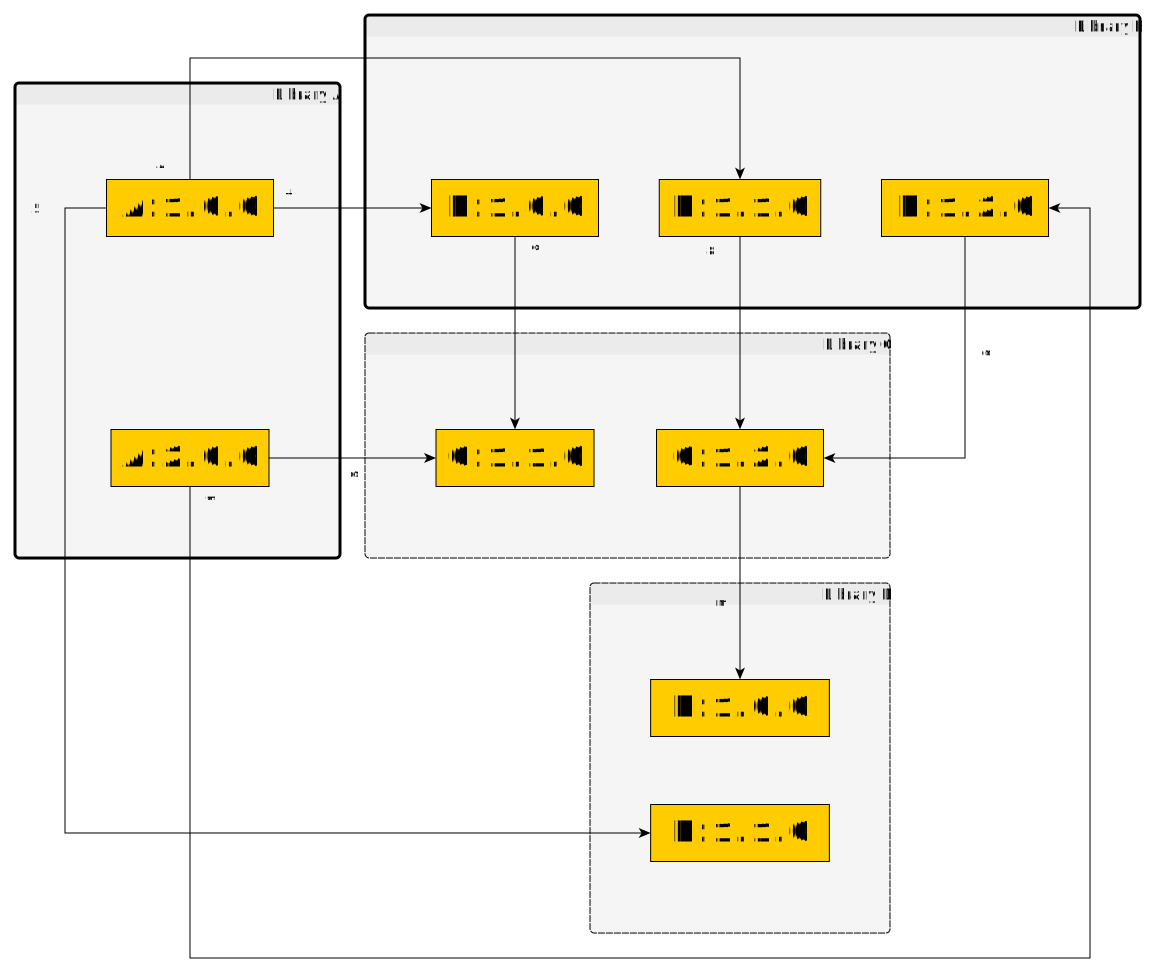
\includegraphics[width=\columnwidth]{fig/complex_case}
  \caption{Graphical representation of package dependencies}\label{fig:deps}
\end{figure}


It should be noted that there are a variety of other special cases we
also deal with like self dependency and cyclic dependency.  But these
are constraints like any other and don't really impact the algorithm
in any significant way.

\subsubsection{Formulating Constraints}

The default assumption is that dependencies will come from the
\code{uses} annotation in Modelica.  There is a proposal to extend the
\code{uses} annotation to allow multiple compatible versions to be
listed (vs.\ only a single compatible version today).  As mentioned
perviously, such an \code{or} relationship is already supported by
\code{impact}.  So this change would not impact the resolution
algorithm used by \code{impact}.

Although it hasn't yet been implemented, one proposed fallback mode
for \code{impact} is to ignore the explicit dependencies contained in
Modelica code and instead rely on the dependency relationships {\bf
  implicit} in semantic versions.  In other words, if a library
\code{B} has two versions, \code{1.1.1} and \code{1.1.2}, and those
versions strictly follow semantic versioning conventions, then we know
that any library that depends on \code{B:1.1.1} must also be
compatible with \code{B:1.1.2}.  Such a fallback mode could be
employed when \code{impact} is unable to find a solution using
explicit constraints.

\section{Go Implementation}

We've created an implementation of \code{impact} using Go~\parencite{go-lang}.
This implementation includes different sub-packages for dealing with
crawling repositories, resolving dependencies, parsing Modelica code
and managing configuration settings.  It also contains a sub-package
for implementing the command-line tool and all of its sub-commands.
This structure means that \code{impact} is not only a command-line
tool, but also a Go library that can be embedded in other tools.

The Go implementation includes the following commands:
\begin{description}[noitemsep]
  \item[\code{search}] Search library names and descriptions for
    search terms.
  \item[\code{install}] Install one or more libraries and their
    dependencies.
  \item[\code{index}] Build an index of repositories.
  \item[\code{version}] Print out version and configuration
    information.
\end{description}

For each command, you can use the \code{-h} switch to find out more
about the command and its options.

Earlier we described our requirements.  The main reason we moved to Go
from Python was Go's support for cross-compiling between all major
platforms and the fact that it generates a statically linked binary
that doesn't depend on any runtime.  The Go compiler includes a
complete implementation of HTTP for both the client and server.  In
fact, the standard library for Go is fairly complete.  At the moment,
the only third party dependencies for \code{impact} are a Go
implementation of the GitHub v3 API and an implementation of semantic
versioning.

The performance of compiled Go code is quite good.  In
Section~\ref{sec:algorithm} we described how the algorithm we are using could,
in a worst case scenario, search every potential combination before
finding either a solution or failing.  We constructed several test
cases with $n$ variables where each variable had $2$ possible values.
The result is that there will be $2^n$ possible combinations.  These
cases were contrived so that the least desirable combination was the
only one that would satisfy the dependency constraints.  We tested the
time required for find a solution for different values of $n$ and we
got the following performance results:

\subsection{Requirements}

\begin{center}
\begin{tabular}{ll}
$n$ & Time (ms) \\
10 & 45 \\
12 & 141 \\
14 & 646 \\
20 & 52,000 \\
\end{tabular}
\end{center}

It is important to keep in mind that this is a {\bf contrived} case to
demonstrate the worst possible case for resolution.  There may very
well be other algorithmic approaches that find identical solutions be
search more efficiently.  But given what we know about Modelica
libraries and their dependencies, we found this performance more than
sufficient for this particular problem.

One last point worth making about the implementation of \code{impact}
has to do with security.  In order to generate an index from GitHub
repositories, it is necessary to crawl repositories.  In order to
accomplish this, many API calls are required.  GitHub will only allow
a very limited number of ``anonymous'' API calls.  This limit will be
reached very quickly by \code{impact}.  In order to increase the
number of allowed API calls, GitHub requires an ``API key'' to be
used.  Such a key can be provided to \code{impact} but it cannot be
provided via a command line option or a configuration file.  This is
to avoid this sensitive information being inadvertently recorded or
exposed (\emph{e.g.,} by committing it to a version control
repository).  Instead, such tokens must be provided as environment
variables.

The \code{impact} source code is licensed under an MIT license and is
hosted on GitHub.  The GitHub repository includes a \code{LICENSE},
\code{README.md} and \code{CONTRIBUTING.md} which provide a details
license, introductory documentation and instructions for contributors,
respectively.  We've linked the GitHub repository to a continuous
integration service so that each commit triggers tests and email out
build status to the maintainers.

\section{\code{impact} on library developers}

What does it mean for library developers wanting to make their library
accessible via \code{impact}? Let us first have a look at the past
``sins'' that were restricting the development work on Modelica
libraries.

\subsection{Observations}
\begin{enumerate}
\item  We noticed that the \texttt{MODELICAPATH} concept is not properly
  understood  by the users and often comes into their way.
Therefore one should not rely on it but rather work with a
\emph{working directory} (which should always part of the
\texttt{MODELICAPATH} and made first priority for the look-up in the
tool).
\item  If we go away from having to collect all Modelica libraries
in the \texttt{MODELICAPATH}  then there is no longer a need to store the
  version number with the library folder name.
I.e., simply ``\texttt{<PackageName>}'' is sufficient and no need for
``\texttt{<PackageName>~<Version>}''.
\item  Until now we advised the lib developers to have the development
  work in a \texttt{master} branch and merge \texttt{master} into a
  \texttt{release} branch where then the directory structure can be
  changed (e.g., into ``\texttt{<PackageName> <Version>}'' and
  generated content can be added) and then finally place the tag on
  the release branch. This has the following effects:
  \begin{description}
  \item[\textbf{+}] The link to the tag will give one a (tar)zip file
    that contains the library with the
    ``\texttt{<PackageName>~<Version>}'' format ready to be used with
    \texttt{MODELICAPATH}. Since we don't want to rely on
    \texttt{MODELICAPATH} any more we don't need to add the
    \texttt{<Version>} identifier to the folder anymore.
  \item[\textbf{-}] If one would like to see what stage a certain
    release in \texttt{master} was then one need to either inspect the
    git history (following backwards from the release tag) or use an
    additional tag (e.g., ``\texttt{1.2.3-dev}'') which is rather
    cumbersome and seems unnecessary.
  \end{description}
\end{enumerate}

\subsection{Repository structure recommendations}
There are new features/mechanisms made available both by GitHub and
\code{impact}:
\begin{itemize}
\item GitHub's support for assets \parencite{gh-assets} allows one to
  upload adtional files to tagged releases
\item  \code{impact} does not use the \texttt{MODELCAPATH} model but
  rather uses a ``one working directory per project'' approach where a
  library of \textbf{one} version  and all dependencies live in one
  (working) directory. A different version of the same library would
  be placed in a different working directory.
  Making these self-contained project folders.
\end{itemize}

Bases on which we recommend that library developers make the most of
it and change the structure in which they organize their library repositories.
\begin{enumerate}
\item Get rid of the \texttt{release} branch as long as it was only
  for the sake of providing a download-able zip-file with a customized
  structure or providing additional generated files.
  Instead use the new GitHub Releases~\parencite{gh-assets} which
  allows uploading of additional assets for download.
  \begin{itemize}
  \item E.g., rather than adding HTML documentation to the
    \texttt{Resources} sub-folder and committing this to the
    \texttt{release} branch and then tagging it, tag the
    \texttt{master} branch and then generate a zip-file which contains
    that state and add the generated files to the tagged release.
    GitHub also provides some information on ``Creating
    Releases''~\parencite{gh-releases} and there exist for example the
    \texttt{aktau/github-release} tool~\parencite{aktau-github-release}
    to help automating that process.
  \item Another benefit of  the assets is that the GitHub
    API~\parencite{gh-api} allows you to get the download count for
    your releases~\parencite{gh-dl-count}.
    This was not possible for the simple taggged-zip-ball downloads.
  \end{itemize}
\item Get rid of the \texttt{<PackageName> <Version>} formatted folder
  names. The version number does not belong in the  \texttt{master}
  (i.e., development)  branch anyway and the version annotation is
  contained  in the \texttt{version} annotation which tools will happily
  display for you. When you install a package with \code{impact} it
  will strip that version number in any case.
\end{enumerate}

\subsection{Changes for the library listing}
The listing of Modelica libraries on
\url{https://modelica.org/libraries} is generated by parsing the
GitHub~API and creating a static HTML file that contains all
information with links. Currently it is a stand-alone \emph{Python}
script but we are thinking of adding this functionality as a
sub-module to \code{impact} itself.

Currently the listing links directly to the (tar)zip-ball URL of the
latest tag of a library. This works fine if the library uses the old
\texttt{release} branch model where the ``ready to install'' version was
placed.  Clicking on that coloured version link will result in a direct file download.

This will be changed in such a way that if one clicks on the listed
``Last Release'' button one will be redirected to the ``Releases'' page of
that project showing the last release. This has the advantage that one
does not immediately downloads the (tar)zip ball but gets to see
proper release notes first \emph{and} is given a choice of what
version of a release one can download (e.g., pure source distribution
of that tag, customised version with additional files, different
platform dependent versions with pre-compiled binaries).

\subsection{Which license is best for your library}
The \emph{Modelica Standard library} (\texttt{Modelica})~\parencite{MSL} is licensed under
the ``Modelica License Version 2.0''~\parencite{MoLic2}. So in order
to stay compatible with the \texttt{Modelica} library most user libraries choose the
same license. This seemed to be just natural. Now there is one problem
which is not very apparent to most library developers. This is that
the ``Modelica License Version 2.0'' contains the section
``4. Designation of Derivative Works and of Modified Works'' which
says that ``\emph{\ldots This means especially that the (root-level)
  name of a Modelica package under this license must be changed if the
  package is modified \ldots}''.
This clause makes perfect sense for a main library like the
\texttt{Modelica} library that is developed and maintained by a major
group centrally and wants to protect its product name.
But what does this mean for open-source projects that no longer are
hosted centrally but rather decentralized on platforms like GitHub and
GitLab but were contributions no longer are made by committing
directly into \textbf{one} central repository? In the de-centralised
case contributions are given by first ``forking'' (i.e., generating a
copy of the original repository), modifying that fork and then sending
the contribution back via a ``pull-request'' (i.e., offering the
originating project to accept the changes made on the fork). Now
already the first step here, the ``forking'', generated a copy with the
identical ``(root-level) name'' and at a different location. One could argue that this
alone is already a violation of the terms of the ``Modelica License
Version 2.0''.

So what should the library developer do? The simplest solution is to
``not'' use the ``Modelica License Version 2.0'' for user libraries
but rather go for standard licenses~\parencite{lic} that are similar
in  nature like, MIT or BSD style license. Interestingly enough the
old ``Modelica License Version 1.1'' is still suitable for user
libraries since it does not contain the restrictions of having to
change the package name.

So what about ``copy-left style'' licenses? The most famous being the
GNU General Pubic license. People might think this
would be a good choice for a license in order
to protect parts of their library being used inside proprietary
libraries without any bugfixes and improvements being fed back to them
as ``upstream'' developers. Unfortunately the GPL also forbids that any
other non-GPL library (even the Modelica Standard Library) uses
the GPL library and being distributed that way. So what about the
LGPL, this allows the usage and distribution \emph{alongside} with
other non-gpl libraries. The problem her is that it does not allow
static linking. Something that happens when one creates a compiled
version of simulation model that uses different Modelica libraries.
A typical example would be the generation of an FMU~\parencite{FMI}.
A way out is here the ``Mozilla Public License'' which is very much
alike the LGPL but allows generated code to be statically linked
together with non-GPL licensed code.

Conclusion. For user libraries should if possible avoid the ``Modelica
License Version 2.0'' as this was primarily designed for the
requirements of the \emph{Modelica Standard library}. Perhaps there
will be a future revision that is adapted to current open-source
development models for user libraries. Until then try to use standard
libraries that are BSD/MIT style.


\section{Future Development}

\subsection{Dependency Constraints}
% These are largely because of limitations in Modelica itself.  Is this
% worth mentioning?  Sure, we frequently go beyond Modelica.  But should
% we worry about this of the language doesn't?
As already mentioned, there is currently no way to express conflicts
between different packages.  However, it is highly likely that such
conflicting pairs will exist as more and more packages are published.
For instance, two Modelica models might depend on different, specific
versions of an external library that cannot be linked or loaded at the
same time, an already published package might contain known bugs etc.
Hence, \code{impact} could be extended by the means to express
conflicts as well.

Boender introduces the notions of \emph{strong dependencies} and
\emph{strong conflicts} to optimize the handling of very large
repositories.  This kind of optimizations might not be necessary in
the Modelica ecosystem right now, but could provide helpful
performance enhancements in future versions of \code{impact}.

\subsection{Crawling}

At the moment, \code{impact} is only able to crawl GitHub
repositories.  There is nothing particularly special about GitHub
and/or its APIs.  The authors are confident that indices could be
constructed for many different storage types.  The most obvious next
steps for crawling support would be to add support for Bitbucket and
Subversion repositories.  Pull requests to introduce such
functionality would be welcome.

On a related note, we anticipate there will be many use cases where
\code{impact} could be useful for closed source projects that involve
private repositories.  We think this is an important use case and we
hope to provide support for crawling such repositories.  This would,
for example, allow model developers at companies that have made a
significant investment in building Modelica related models and
libraries to use \code{impact} to search and install these proprietary
libraries via the corporate intranet.

\subsection{Project Details}

We have already created a number of issues that require users to
provide more explicit information about how they want impact to
function on a per project bases.  For example, when working with
forked libraries (where the index contains multiple libraries with the
same name), it is useful to use the URIs associated with each library
in the index to disambiguate which particular library to use.
Furthermore, there may be cases where the user is actually interested
in making changes to the dependencies.  In such cases, those
dependencies shouldn't simply be installed, they should be {\bf
  checked out} from their repository to make modification and
re-committing easier.

For these and other project related features, we feel there is a need
to introduce another file to provide such additional information.

\subsection{Web Based Search}

Other package managers often provide a web site where users can search
for a specific package through the web, read documentation, log issues
and/or even download the packages.  Because \code{impact} is organized
into libraries (and not just a command line tool), we feel this kind
of functionality could be added in the future.

\subsection{Installers}

Finally, when installing software, it is common for developers to
distribute ``installers'' (\emph{i.e.,} executables that, when run,
unpack and install the software).  Another potential extension of
\code{impact} could be to generate such installers.  In this case, we
could once again leverage Go's static executable generation to build
such installers from the index.  Instead of installing the needed
files locally, the installer could simply bundle them up and attach
them to an installation program using one of the many Go
extensions~\parencite{GeertJohan/go.rice,tebeka/nrsc}
for concatenating static content onto executables or simply
downloading some pre-specified libraries over the network.

\section{Conclusion}

In conclusion, \code{impact} leverage information already available in
Modelica source code along with some common conventions in order to
help users find and install Modelica libraries.  It does this by
crawling repositories and indexing their contents.  An index of
publicly available libraries created by \code{impact} is hosted on
\code{modelica.org}.

If present, the \code{impact} command line tool is already used by
OpenModelica to help find and install dependencies.  By making the
\code{impact} executables available across platforms and providing a
version of the source code that can also be embedded as a library, we
hope the Modelica community will benefit from having first class
package management capabilities, just like other software eco-systems.

\section{Acknowledgements}
\label{sec:acknowledgements}

The authors would like to thank
\href{mailto:christoph.hoeger@tu-berlin.de}{Christoph H\"oger} of
Technische Universit\"at Berlin,
\href{mailto:martin.sjolund@liu.se}{Martin Sj\"olund} of Link\"oping
University, \href{mailto:francesco.casella@polimi.it}{Francesco Casella}
of Politecnico di Milano and \href{mailto:Peter.Harman@esi-group.com}
{Peter Harman} of ESi Group for their contributions to this project.

%%% Remove the following line once we got real citations in place.
%\nocite{*}
%--------------------------------------------------------------------------------
% References using biblatex
\small
\printbibliography%
\normalsize

\end{document}
